%Only use subsection and subsubsection
The aim of this project is to allow the robot to be able to learn movement from demonstrations.\\
In this report, we presented the trajectory processing componenent which is the transformation of a demonstration to simple commands on how the robot need to adapt its trajectory.\\

Here are some steps of the process, the operator applies a kinestethic correction on the robot while doing a movement. This demonstration is provided to an algorithm which isolates the correction using the data (velocity and original trajectory), then transforms the correction into a continuous curve (cubic splines) and finally, when moving again near the same place where the correction was applied, it gets aligned to the shown correction. A continuous Gaussian Process Regression is used by computing a distance from the actual position of the robot to the correction curve.\\

In this project, algorithms were developed on Matlab and implemented on the robot using ROS library in Python. The codes can all be found in a private repository:\\
\url{https://github.com/epfl-lasa/nl-dynamics}


\paragraph*{Discussion}

The main developement towards the robotics in this project concerns the continuous Gaussian Process Regression adaptation. Indeed this algorithm provides a robust data estimation solution from a continuous representation of data. It is used and adapted for splines in this application, however it could be generalized for any continuous representation of data. Indeed, the key of this algorithm is the minimal distance from a point to the curve computation, which could be generalized by a numerical solution.

\paragraph*{Work on the robot}

Finally we tested everything, and the robot learned and moved. Cyril Schmitt has also been working on this project but on the vocal part. When assembling both of our projects, interaction, movement and learning processes of the robot work and gave good results. We were able to control the robot using natural language, and after applying correction and running the learning algorithm, the robot corrected its trajectory itself, see \autoref{Robotsdata}, this graph data's directly comes from the robot. In a 3D space it successfully isolates two corrections from a demonstration.

\begin{figure}[H]
\centering
\fbox{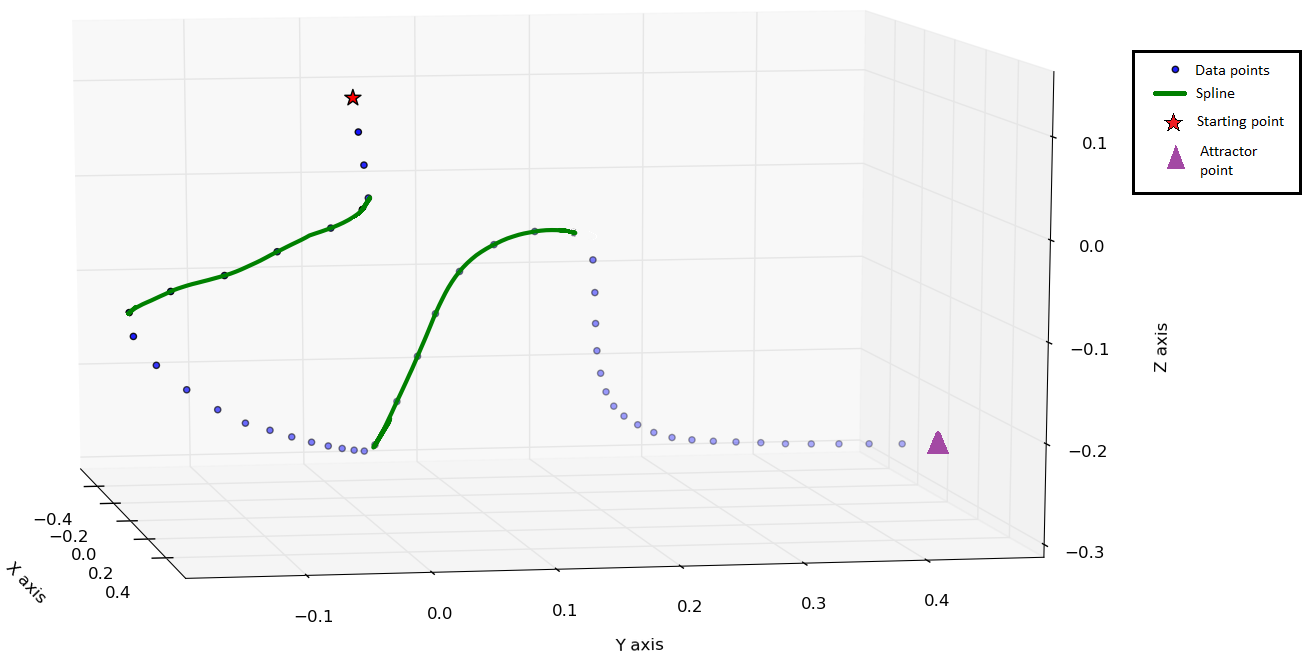
\includegraphics[width=15cm]{img/3d_data.png}}
\caption{3D graph of real robot's data. There are two corrections in the demonstration transform in a continuous curve (spline) in green. The starting point is the red star and the attractor point is the purple triangle.}
\label{Robotsdata}
\end{figure}

\paragraph*{Future work}

Some more tests could have been done for the analysis of the isolation correction algorithm, indeed the precision factor of this algorithm can be tuned more precisely. Also, some improvements could be done such as optimization of the algorithms (the research of the closest point on many cubic splines for example) or developping a concept of showing many times the same correction to the robot to have a better learning, algorithms like putting together many corrections in a 3D space would be developped. However, the project is working and the only future work would concern optimization.\\
